% Bản review tiếng Việt: giữ nguyên nội dung và font, không áp dụng giới hạn trang.
\documentclass[conference]{IEEEtran}
\IEEEoverridecommandlockouts
\usepackage[T5]{fontenc}
\usepackage[utf8]{inputenc}
\usepackage[vietnamese]{babel}
\usepackage{times}
\usepackage{graphicx}
\usepackage{amsmath,amssymb}
\usepackage{booktabs}
\usepackage{array}
\usepackage{url}
\usepackage{balance}
\title{An Automatic Emergency Braking System in CARLA Using Radar--Camera Fusion and Staged PID Control}
\author{
\IEEEauthorblockN{Mai Việt Hoàng và Phạm Đức An}
\IEEEauthorblockA{
\textit{Đại học Bách khoa Hà Nội}\\
Hà Nội, Việt Nam\\
hoangmai04222@gmail.com
}
}
\begin{document}
\maketitle
\begin{abstract}
Phanh khẩn cấp tự động không chỉ cần phát hiện vật thể phía trước, mà còn phải xác định đúng mục tiêu có nguy cơ va chạm với xe ego và can thiệp đủ sớm để tránh phanh muộn hoặc phanh nhầm với xe làn bên. Bài báo trình bày một hệ thống AEB được xây dựng và đánh giá trong môi trường CARLA 0.9.11. Hệ thống sử dụng radar phía trước làm nguồn đo chính cho khoảng cách và vận tốc tương đối; từ đó tính toán TTC và các đại lượng rủi ro. Dữ liệu radar được xử lý ở mức đối tượng thông qua lọc điểm, gom cụm và theo dõi qua nhiều khung hình. Các mục tiêu radar sau đó được kiểm tra theo hành lang quỹ đạo dự đoán của xe ego để loại bỏ các vật thể không nằm trên hướng di chuyển. Camera RGB và YOLO26n được dùng như một tầng xác nhận ngữ nghĩa: mục tiêu radar được chiếu lên ảnh và được chấp nhận khi liên kết hợp lệ với bounding box của lớp xe. Trên cơ sở mục tiêu đã chọn, hệ thống kết hợp TTC, khoảng cách dừng và biên khoảng cách để tạo lệnh phanh bằng bộ điều khiển PID phân tầng. Các bài kiểm thử được xây dựng theo hướng lấy cảm hứng từ các kịch bản AEB car-to-car của NCAP, đồng thời bổ sung một số tình huống mở rộng như xe làn bên, đường cong và cut-in. Kết quả trên 66 kịch bản cho thấy hệ thống đạt 38/38 trường hợp trong dải thiết kế, 25/28 trường hợp kiểm thử giới hạn và 63/66 trường hợp trên toàn bộ tập đánh giá. Ba trường hợp va chạm được giữ lại để phân tích giới hạn ở tốc độ cao, khoảng cách ban đầu nhỏ và tình huống cut-in muộn. Các kết quả này là bằng chứng trong mô phỏng, không phải chứng nhận NCAP hoặc kiểm định trên xe thật.
\end{abstract}
\begin{IEEEkeywords}
phanh khẩn cấp tự động, AEB, hợp nhất camera--radar, CARLA, TTC, PID, ADAS
\end{IEEEkeywords}

\section{Giới thiệu}
Các hệ thống hỗ trợ lái xe nâng cao (ADAS) quan sát môi trường, đánh giá rủi ro và cảnh báo hoặc can thiệp điều khiển để giảm khả năng va chạm. AEB đặc biệt quan trọng vì không chỉ cảnh báo mà còn trực tiếp tạo lệnh phanh khi người lái không phản ứng kịp. Các tình huống xe trước đứng yên, xe trước chạy chậm hơn và xe trước phanh gấp là những nhóm cốt lõi trong đánh giá AEB xe--xe \cite{euroncap_aeb,iso15623}.

AEB không thể chỉ phanh theo vật thể gần nhất. Radar đo tốt khoảng cách và vận tốc tương đối nhưng tín hiệu thưa, có thể chứa phản xạ từ mặt đường, lan can hoặc xe làn bên. Camera nhận biết hình dạng đối tượng tốt hơn nhưng không trực tiếp đo vận tốc đóng. Vì vậy hệ thống cần trả lời đồng thời: vật thể có phải xe không; có nằm trong đường đi dự kiến của ego không; và còn đủ thời gian hoặc quãng đường để phanh không.

Thử nghiệm gần va chạm trên xe thật cần bãi thử, mục tiêu giả, thiết bị đo và quy trình an toàn nghiêm ngặt. CARLA là môi trường mô phỏng cung cấp cảm biến, actor giao thông, điều khiển đồng bộ và nhãn chuẩn để lặp lại cùng kịch bản trong điều kiện có kiểm soát \cite{dosovitskiy2017carla,carla_docs}. Bài báo xây dựng pipeline AEB trên CARLA 0.9.11 với Tesla Model 3, một camera RGB và một radar phía trước.

Đóng góp của bài báo gồm: 1) pipeline radar mức đối tượng có lọc theo hành lang quỹ đạo và xác nhận đa khung hình; 2) fusion gate hình học radar--YOLO chỉ dùng dữ liệu online, không dùng actor ID hay ground truth CARLA để ra quyết định; và 3) tích hợp lựa chọn mục tiêu, fusion gate, TTC, khoảng cách dừng và staged PID thành pipeline AEB end-to-end, được đánh giá trên miền thiết kế và các kịch bản kiểm thử giới hạn. CCRs, CCRm và CCRb lấy cảm hứng từ NCAP; cut-in, đường cong, xe làn bên và nhiều xe là kiểm tra kỹ thuật bổ sung.

Các kết quả trong bài báo được diễn giải trong phạm vi mô phỏng CARLA và dùng để đánh giá nội bộ pipeline đề xuất; chúng không phải chứng nhận an toàn, chứng nhận NCAP hoặc kiểm định trên xe thật.

Phần còn lại của bài báo được tổ chức như sau. Mục II tóm tắt các công trình và tiêu chuẩn liên quan. Mục III xác định phạm vi mô phỏng, các giả định và nguyên tắc không dùng ground truth khi hệ thống ra quyết định. Mục IV trình bày pipeline đề xuất. Mục V mô tả thiết kế thực nghiệm, bộ kịch bản và tiêu chí đánh giá. Mục VI phân tích kết quả cuối cùng, gồm các tình huống đạt, các tình huống không đạt và ý nghĩa của chúng đối với giới hạn hoạt động.

\section{Công trình liên quan}
CARLA được sử dụng rộng rãi trong nghiên cứu xe tự hành nhờ khả năng cấu hình bản đồ, thời tiết, phương tiện, cảm biến và synchronous simulation \cite{dosovitskiy2017carla,carla_sensors}. Radar và camera là hai nguồn bổ sung: radar đo khoảng cách/vận tốc xuyên tâm, còn camera cung cấp thông tin ngữ nghĩa. Nhiều phương pháp fusion liên kết dữ liệu qua hiệu chuẩn hình học trước khi theo dõi hoặc ra quyết định \cite{feng2021multimodal}. Bài báo này dùng phép chiếu hình học minh bạch làm \textit{gate} xác nhận, chưa tuyên bố là bộ lọc đa cảm biến xác suất.

YOLO là bộ phát hiện một giai đoạn, dự đoán trực tiếp bounding box, lớp và độ tin cậy, phù hợp cho pipeline thời gian thực \cite{ultralytics_yolo}. Trong hệ thống đề xuất, YOLO chỉ xác nhận lớp car; radar vẫn cung cấp khoảng cách, vận tốc tương đối, TTC và khoảng cách dừng. TTC chỉ hữu ích khi mục tiêu đang tiến lại gần; do đó cần kết hợp TTC với mô hình khoảng cách dừng và biên an toàn \cite{iso15623}. Giá trị của bài báo nằm ở việc tích hợp các khối này thành pipeline có thể chạy, ghi log và đánh giá.

\section{Phạm vi và giả định mô phỏng}
Bài toán được giới hạn trong miền vận hành thiết kế (ODD) hẹp để có thể đánh giá chặt chẽ. Xe ego chạy trên đường cao tốc trong Town04, thời tiết và ánh sáng lý tưởng, đối tượng quan tâm là ô tô phía trước hoặc ô tô nhập làn trước ego. Dải vận tốc chính là 50--80 km/h; các trường hợp 95--110 km/h hoặc gap rất ngắn được xem là stress test. Cách phân tách này tránh việc một tỷ lệ pass chung che mất thông tin quan trọng: hệ thống có thể hoạt động tốt trong ODD nhưng vẫn có giới hạn rõ khi tốc độ cao hoặc target xuất hiện quá muộn.

Trong simulator, CARLA có thể cung cấp nhiều thông tin hoàn hảo như actor ID, vị trí actor, bounding box 3D và collision event. Dự án chỉ dùng các thông tin này ở ba nơi không tham gia quyết định online: sinh nhãn YOLO offline, tạo thống kê đánh giá, và kiểm chứng video/log sau khi chạy. Khi hệ thống đang quyết định phanh, đầu vào chỉ gồm ảnh RGB, điểm radar, trạng thái xe ego và kết quả xử lý từ các module perception. Do đó kết quả phản ánh năng lực của pipeline cảm biến mô phỏng, không phải một thuật toán được gợi ý bởi nhãn chuẩn của simulator.

Giả định động lực học cũng được giữ ở mức phục vụ nghiên cứu. Mô hình không xét trượt bánh, ma sát thay đổi, ABS chi tiết, độ trễ thủy lực phanh hay mô hình lốp đầy đủ. Tác động phanh được CARLA mô phỏng qua control command. Vì vậy các đại lượng như khoảng cách nhỏ nhất, TTC, thời điểm bắt đầu phanh và collision là đáng tin trong phạm vi so sánh nội bộ giữa các kịch bản, nhưng không nên chuyển trực tiếp thành thông số thiết kế cho xe thật.

\section{Phương pháp đề xuất}
\subsection{Kiến trúc và xử lý radar}
Luồng xử lý online gồm: cảm biến CARLA $\rightarrow$ radar object $\rightarrow$ YOLO $\rightarrow$ fusion gate $\rightarrow$ chọn target $\rightarrow$ TTC/khoảng cách dừng $\rightarrow$ staged PID $\rightarrow$ ghi đè lệnh điều khiển. Hình~\ref{fig:sensor} cho thấy bố trí camera sau kính lái và radar ở mũi xe. Mô phỏng chạy tick cố định 20 Hz; chỉ số định lượng lấy từ log mô phỏng thay vì FPS hiển thị.

Về mặt chức năng, radar đóng vai trò đo động học, camera đóng vai trò xác nhận ngữ nghĩa, còn bộ điều khiển phanh chỉ nhận một target hợp lệ. Thiết kế này cố ý giữ các giao diện trung gian dễ kiểm tra: radar object có thể xem trong bird-eye view, YOLO box có thể xem trên ảnh, fusion decision có thể giải thích bằng việc điểm radar chiếu vào hoặc không chiếu vào box xe, và AEB state có thể đối chiếu với TTC/khoảng cách dừng trong biểu đồ log. Khả năng truy vết này quan trọng với đồ án nghiên cứu vì giúp phân biệt lỗi perception, lỗi target selection và lỗi điều khiển.

\begin{figure}[t]
\centering
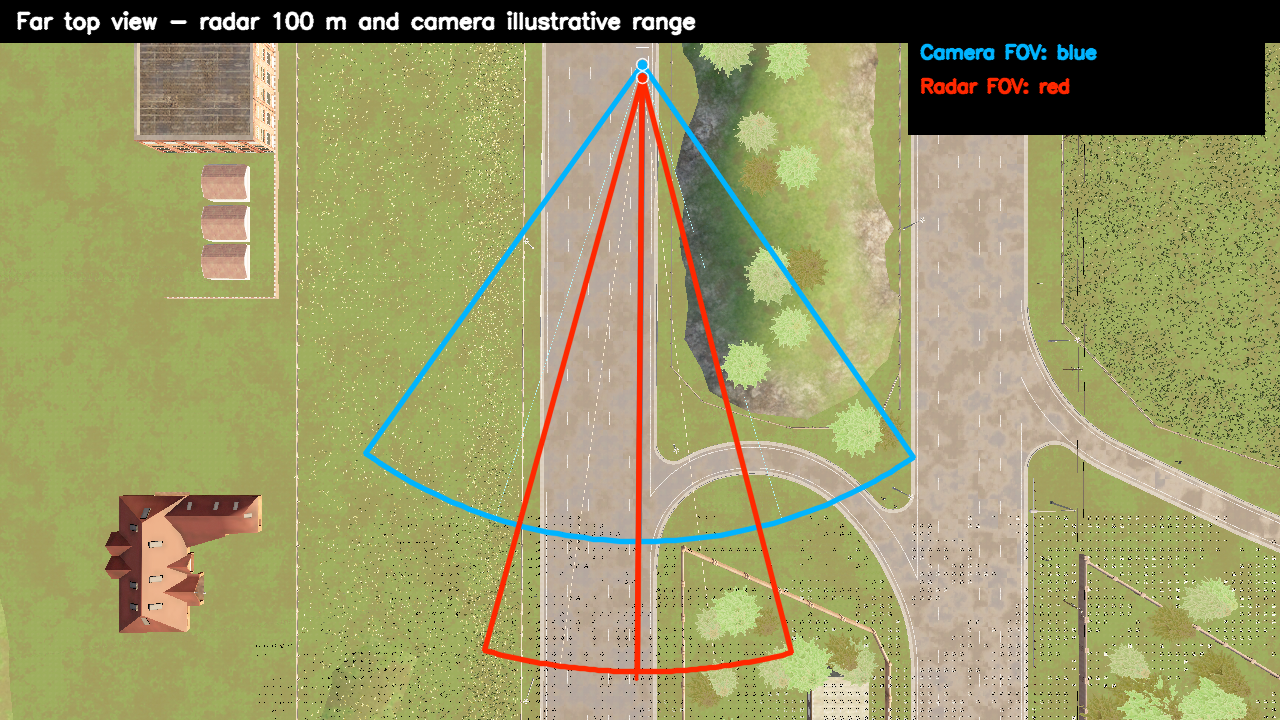
\includegraphics[width=\columnwidth]{../../report/assets/evidence/sensor_far_top_view.png}
\caption{Vùng quan sát của camera RGB và radar phía trước trên xe ego.}
\label{fig:sensor}
\end{figure}

Mỗi điểm radar có khoảng cách dọc $x$, lệch ngang $y$, độ cao $z$, vận tốc tương đối $v_r$ và vị trí thế giới. Pipeline loại điểm ngoài tầm radar, quá thấp gần mặt đường, quá cao hoặc quá xa hành lang dự đoán. Các điểm còn lại được gom cụm khi khoảng cách phẳng, chênh cao và chênh vận tốc cùng nhỏ hơn ngưỡng cấu hình. Trong mỗi cụm, $x$ lấy percentile 20\% nhằm tránh bị kéo xa bởi điểm phía sau; $y$, $z$ và $v_r$ lấy median để tăng tính bền vững với nhiễu.

Tracker dự đoán vị trí track theo vận tốc tương đối, ghép measurement mới với track cũ theo khoảng cách và vận tốc, sau đó yêu cầu track tồn tại liên tiếp qua nhiều frame trước khi gắn cờ \textit{confirmed}. Đầu ra gồm khoảng cách dọc, lệch ngang, vận tốc tương đối, số điểm, độ tin cậy, tuổi track và TTC. Object được chọn ưu tiên TTC hữu hạn nhỏ nhất, sau đó theo khoảng cách dọc nhỏ nhất. Như vậy, điểm radar đơn lẻ hoặc object xuất hiện thoáng qua không thể trực tiếp gây phanh.

Một khó khăn thực tế là radar thường phát hiện nhiều điểm trên cùng một xe, trong khi AEB chỉ cần một đại diện ổn định của vật thể nguy hiểm. Nếu lấy điểm gần nhất tuyệt đối, nhiễu hoặc phản xạ ở mép xe có thể làm TTC dao động. Nếu lấy trung bình đơn giản, cụm radar có thể bị kéo bởi điểm ở phía sau xe hoặc điểm ngoài thân xe. Bởi vậy pipeline dùng percentile/median cho vị trí và vận tốc, sau đó dùng tracking đa khung hình để làm mượt. Cách làm này không phức tạp như lọc Kalman đầy đủ, nhưng đủ minh bạch và dễ debug trong bối cảnh một xe ego, một hoặc vài target phía trước.

Hành lang lọc radar được áp dụng trước target selection. Những object có lệch ngang lớn so với đường đi dự đoán sẽ bị loại ngay cả khi khoảng cách dọc nhỏ. Đây là cơ chế chính để xử lý xe làn bên và xe mồi trong kịch bản nhiều actor. Nếu chỉ dựa vào khoảng cách radar, các xe làn bên đứng yên có thể bị coi là nguy hiểm vì có $d$ nhỏ và $v_c$ lớn khi ego đi qua; hành lang quỹ đạo giúp gắn quyết định phanh với không gian mà ego thực sự sẽ đi qua.

\subsection{YOLO và fusion gate hình học}
YOLO26n được fine-tune cho một lớp \textit{car}. Dataset cuối có 1.505/300/200 ảnh train/validation/test và 1.872/379/264 bounding box. Nhãn được tạo offline bằng cách chiếu bounding box 3D của actor CARLA lên ảnh, kiểm tra phần xe nhìn thấy và xuất nhãn YOLO. Ground truth chỉ dùng để tạo dữ liệu; tại runtime pipeline không truy cập actor ID, semantic label hay bounding box chuẩn. Với ảnh $640\times640$, mô hình huấn luyện 100 epoch đạt precision 0,9919, recall 0,9642, $\mathrm{mAP}_{50}$ 0,9940 và $\mathrm{mAP}_{50:95}$ 0,9495 ở epoch tốt nhất.

Quy trình tạo dữ liệu chọn cùng góc nhìn camera với runtime để giảm lệch miền dữ liệu. Mỗi ảnh được tạo nhãn từ actor trong CARLA, sau đó chỉ giữ các box hợp lệ cho lớp car. Cách này nhanh hơn gán nhãn thủ công và cho phép thu nhiều case theo vận tốc/gap khác nhau, nhưng cũng tạo một giới hạn: mô hình học khá sát môi trường Town04 và điều kiện lý tưởng. Vì vậy trong bài báo, kết quả YOLO được dùng như bằng chứng rằng detector đủ tốt cho vai trò xác nhận trong mô phỏng hiện tại, chưa phải bằng chứng tổng quát cho mọi map, thời tiết hoặc kiểu phương tiện.

\begin{table}[t]
\caption{Tóm tắt dữ liệu và cấu hình nhận thức dùng trong bài báo.}
\label{tab:perception}
\centering
\footnotesize
\begin{tabular}{p{0.37\columnwidth}p{0.46\columnwidth}}
\toprule
Thành phần & Giá trị / vai trò \\
\midrule
Simulator & CARLA 0.9.11, synchronous tick 20 Hz \\
Xe ego & Tesla Model 3, camera RGB trước và radar trước \\
Ảnh YOLO & 640$\times$640, một lớp \textit{car} \\
Dataset & 1.505 train, 300 validation, 200 test \\
Nhãn & 1.872/379/264 box cho train/validation/test \\
YOLO tốt nhất & Precision 0,9919; recall 0,9642; mAP50 0,9940 \\
Fusion & Chiếu object radar lên ảnh và kiểm tra trong bbox YOLO \\
Ground truth runtime & Không dùng actor ID hoặc bbox chuẩn để ra quyết định \\
\bottomrule
\end{tabular}
\end{table}

Điểm radar được biến đổi từ hệ radar qua world sang hệ camera. Với tọa độ camera $(X_c,Y_c,Z_c)$ và $Z_c>0$, điểm ảnh được tính bởi
\begin{equation}
u=f_x\frac{X_c}{Z_c}+c_x,\qquad v=f_y\frac{Y_c}{Z_c}+c_y.
\label{eq:projection}
\end{equation}
Trong đó $f_x=f_y=W/[2\tan(\mathrm{FOV}/2)]$ và $(c_x,c_y)$ là tâm ảnh. Radar object được xác nhận nếu điểm chiếu thuộc bounding box YOLO lớp xe:
\begin{equation}
x_1\leq u\leq x_2,\qquad y_1\leq v\leq y_2.
\label{eq:association}
\end{equation}
Cửa sổ giữ xác nhận 0,35 s giảm ảnh hưởng lệch thời gian giữa camera, radar và suy luận YOLO. Khi radar yêu cầu phanh nhưng target chưa được camera xác nhận, fusion gate nhả lệnh phanh. Cơ chế này giảm false positive, đổi lại có nguy cơ bỏ sót nếu YOLO mất detection hoặc hiệu chuẩn lệch.

Trong thiết kế này, fusion không tạo một object trạng thái mới với hiệp phương sai như các phương pháp object-level fusion xác suất. Nó hoạt động như một cổng xác nhận độc lập: radar phải nói có nguy cơ động học, camera phải nói điểm đó thuộc xe. Ưu điểm là quyết định dễ giải thích, ít tham số và phù hợp với dữ liệu mô phỏng có một radar phía trước. Nhược điểm là hệ thống có thể bảo thủ quá mức trong các frame camera bị mất detection; cửa sổ giữ xác nhận 0,35 s được dùng để giảm hiện tượng nhấp nháy nhưng không thể thay thế tracking đa cảm biến đầy đủ.

\subsection{Quỹ đạo dự đoán, TTC và khoảng cách dừng}
Hành lang quỹ đạo được xây dựng từ tốc độ ego, yaw rate và góc lái để loại xe làn bên. Với độ cong $\kappa$, điểm cách ego một cung $s$ có dạng
\begin{equation}
x(s)=\frac{\sin(\kappa s)}{\kappa},\qquad y(s)=\frac{1-\cos(\kappa s)}{\kappa},
\label{eq:path}
\end{equation}
và chuyển sang đường thẳng khi $\kappa$ gần bằng không. Object ngoài ngưỡng lệch ngang của hành lang bị loại khỏi candidate target.

Theo quy ước của hệ thống, $v_r<0$ nghĩa là target tiến lại gần ego. Vận tốc đóng và TTC là
\begin{equation}
v_c=-v_r,\qquad \mathrm{TTC}=\frac{d}{v_c},\quad v_c>0.
\label{eq:ttc}
\end{equation}
Nếu $v_c\leq0$, TTC là vô hạn. Khoảng cách dừng yêu cầu được tính:
\begin{equation}
d_{req}=\max\left(d_0,v_e t_r+\frac{v_e^2}{2a_e}-\frac{v_t^2}{2a_t}+d_0\right).
\label{eq:stopping}
\end{equation}
Trong đó $v_e,v_t$ là tốc độ ego/target, $t_r$ là thời gian phản ứng giả định, $a_e,a_t$ là gia tốc hãm giả định và $d_0$ là khoảng cách dự phòng. Biên an toàn $d_{margin}=d-d_{req}$ giúp kích hoạt phanh khi TTC chưa đủ thấp nhưng quãng đường đã thiếu.

\subsection{Máy trạng thái và staged PID}
Máy trạng thái giám sát có bốn trạng thái NORMAL, WARNING, BRAKE và RELEASE. Trong BRAKE, các mức soft, medium, hard và emergency giới hạn lực phanh tối đa tăng dần. Target phải được tracker xác nhận và ổn định qua target gate, trừ khi khoảng cách hoặc biên khoảng cách quá nguy hiểm. PID dùng sai số khoảng cách và TTC:
\begin{equation}
\begin{aligned}
e_d&=\max(0,d_{th}-d_{margin}-d_{deadband}),\\
e_{ttc}&=\max(0,TTC_{brake}-TTC),\\
e&=e_d+k_{ttc}e_{ttc},
\end{aligned}
\label{eq:error}
\end{equation}
sau đó sinh lệnh
\begin{equation}
b=\mathrm{clip}(b_{min}+K_pe+K_i\!\int e\,dt+K_d\dot e,b_{min},b_{max}).
\label{eq:pid}
\end{equation}
Lệnh tiếp tục bị giới hạn theo tầng rủi ro và rate limiter. Do đó trong tình huống thường phanh tăng dần, còn EMERGENCY cho phép tăng nhanh tới 1,0. Hysteresis giữ phanh tối thiểu 0,3 s và chỉ nhả khi TTC/quãng đường phục hồi.

Bảng~\ref{tab:pidparam} liệt kê các hằng số chính của bản staged PID cuối cùng. Ý tưởng của bảng này không phải tối ưu toàn cục, mà cho thấy cấu hình có thể đọc được và kiểm chứng được. Các ngưỡng hard/emergency theo TTC và margin quyết định khi nào PID được phép đi vào vùng phanh mạnh; các tham số $K_p,K_i,K_d$ quyết định mức tăng trong vùng đó. Việc đặt $K_d=0$ giúp giảm nhạy với đạo hàm nhiễu của khoảng cách/TTC ở tick rời rạc.

\begin{table}[t]
\caption{Một số tham số chính của staged PID.}
\label{tab:pidparam}
\centering
\footnotesize
\begin{tabular}{lll}
\toprule
Nhóm & Tham số & Giá trị \\
\midrule
Staged brake & soft / medium / hard & 0,55 / 0,75 / 0,90 \\
Staged brake & emergency & 1,00 \\
TTC gate & hard / emergency & 1,10 s / 0,80 s \\
Margin gate & hard / emergency & -2,0 m / -5,0 m \\
PID gain & $K_p,K_i,K_d$ & 0,12 / 0,01 / 0,00 \\
PID gain & $k_{ttc}$ & 0,12 \\
PID bound & min / max brake & 0,25 / 1,00 \\
Comfort & target margin & 4,0 m \\
\bottomrule
\end{tabular}
\end{table}

So với phanh nhị phân, staged PID có hai lợi thế trong thí nghiệm. Thứ nhất, nó tránh việc nhảy ngay lên phanh cực đại trong các tình huống mới ở mức cảnh báo hoặc soft, giúp biểu đồ lệnh phanh dễ quan sát hơn. Thứ hai, khi target thực sự nguy hiểm, máy trạng thái vẫn cho phép tăng nhanh lên hard hoặc emergency. Nói cách khác, tầng trạng thái quyết định mức rủi ro, còn PID quyết định lượng phanh bên trong mức đó.

\section{Thiết kế thực nghiệm}
Môi trường dùng Town04, Tesla Model 3, thời tiết lý tưởng, camera RGB sau kính lái và radar ở mũi xe. Một scenario nguy hiểm PASS khi AEB can thiệp và không xảy ra collision; scenario không nguy hiểm PASS khi không có phanh nhầm. Mỗi tick ghi collision, target, TTC, khoảng cách, vận tốc ego, lệnh phanh và khoảng cách nhỏ nhất. Video chỉ minh họa; kết luận định lượng dựa trên log synchronous 20 Hz.

Các chỉ số chính gồm: \textit{collision}, khoảng cách nhỏ nhất giữa ego và target, vận tốc ego tại thời điểm bắt đầu phanh, gap tại thời điểm bắt đầu phanh, trạng thái AEB theo thời gian và lệnh phanh. Với kịch bản không nguy hiểm, chỉ số quan trọng là false brake: nếu xe làn bên hoặc xe mồi làm AEB phanh dù đường ego không bị cản, case bị tính không đạt. Với kịch bản nguy hiểm, hệ thống phải vừa phát hiện target đúng vừa tạo phanh đủ sớm để collision flag của CARLA không bật.

Tất cả kịch bản được chạy bằng batch script để giữ cùng cấu hình cảm biến, mô hình YOLO, thuật toán fusion và tham số staged PID. Điều này làm kết quả dễ tái lập hơn so với chạy thủ công từng video. Sau mỗi scenario, log CSV và summary JSON được sinh tự động; biểu đồ phanh được tạo từ log để kiểm tra trực quan thời điểm phanh, tốc độ, TTC và vùng trạng thái. Khi có mâu thuẫn giữa cảm nhận video và số liệu, bài báo ưu tiên số liệu log vì video có thể bị ảnh hưởng bởi góc nhìn camera hoặc tốc độ phát lại.

Tập cuối gồm 66 case: đường trống; CCRs, CCRm, CCRb; xe làn bên; đường cong; cut-in/cut-out; và nhiều actor. Bảng~\ref{tab:scope} phân tách hai lớp đánh giá. Nhóm đầu kiểm tra dải hoạt động mục tiêu; nhóm sau mở rộng tốc độ, gap và độ khó để tìm giới hạn, không nhằm làm đẹp tỷ lệ pass.

\begin{table}[t]
\caption{Hai lớp kịch bản và cách diễn giải kết quả.}
\label{tab:scope}
\centering
\footnotesize
\begin{tabular}{p{0.19\columnwidth}p{0.36\columnwidth}p{0.30\columnwidth}}
\toprule
Nhóm & Điều kiện điển hình & Mục đích \\
\midrule
Miền thiết kế & Cao tốc, xe ô tô, thời tiết lý tưởng, chủ yếu 50--80 km/h & Xác nhận dải hoạt động mục tiêu \\
Stress test & 95--110 km/h, gap ngắn, CCRb gắt, cut-in khó & Tìm giới hạn hệ thống \\
\bottomrule
\end{tabular}
\end{table}

Bảng~\ref{tab:scenariofamilies} mô tả các nhóm scenario chính. CCRs, CCRm và CCRb dùng để kiểm tra năng lực car-to-car cơ bản. Cut-in/cut-out kiểm tra việc target xuất hiện hoặc rời khỏi hành lang ego. Adjacent-lane và curve kiểm tra false positive khi radar thấy vật thể gần nhưng đường đi của ego không cắt qua vật thể đó. Multi-actor kiểm tra việc chọn đúng xe nguy hiểm khi có nhiều phản xạ/detection cùng lúc.

\begin{table}[t]
\caption{Các họ kịch bản dùng trong tập đánh giá cuối.}
\label{tab:scenariofamilies}
\centering
\footnotesize
\begin{tabular}{p{0.25\columnwidth}p{0.55\columnwidth}}
\toprule
Họ kịch bản & Vai trò trong đánh giá \\
\midrule
Clear road & Kiểm tra hệ thống không tự phanh khi không có nguy hiểm \\
CCRs & Ego tiến tới xe đứng yên cùng làn \\
CCRm & Ego tiến tới xe trước chạy chậm hơn \\
CCRb & Xe trước đang chạy rồi phanh gấp \\
Cut-in/cut-out & Target nhập làn hoặc rời làn trước ego \\
Adjacent lane & Xe làn bên không được gây phanh nhầm \\
Curve & Kiểm tra hành lang quỹ đạo trên đường cong \\
Multi-actor & Kiểm tra chọn đúng target giữa xe mồi và xe nguy hiểm \\
\bottomrule
\end{tabular}
\end{table}

Một điểm cần nhấn mạnh là tập stress test không bị loại khỏi báo cáo. Ngược lại, các case thất bại được giữ lại vì chúng cho thấy hệ thống còn thiếu gì. Với một bài nghiên cứu, việc chỉ báo cáo các case đạt dễ làm kết quả thiếu tính khoa học. Các thất bại ở CCRb tốc độ cao và cut-in muộn giúp xác định vùng cần cải tiến: phát hiện sớm hơn, dự đoán hành vi target tốt hơn, hoặc điều khiển phanh mạnh hơn trong điều kiện rất gấp.

\section{Kết quả và thảo luận}
Bảng~\ref{tab:results} là kết quả pipeline cuối gồm YOLO ONNX, radar object pipeline, fusion gate và staged PID. Hệ thống đạt toàn bộ 38 case miền thiết kế. Khi mở rộng sang 28 stress case, hệ thống đạt 25 case; ba va chạm được giữ lại. Kết quả toàn bộ là 63/66, tương đương 95,45\%.

\begin{table}[t]
\caption{Kết quả final evidence của hệ camera--radar và staged PID.}
\label{tab:results}
\centering
\footnotesize
\begin{tabular}{lrrr}
\toprule
Nhóm đánh giá & Số case & PASS & FAIL \\
\midrule
Miền thiết kế & 38 & 38 & 0 \\
Stress test/tìm giới hạn & 28 & 25 & 3 \\
\midrule
Tổng cộng & 66 & 63 & 3 \\
\bottomrule
\end{tabular}
\end{table}

Bảng~\ref{tab:cases} liệt kê các case đại diện được dùng để phân tích sâu. Các giá trị ``brake speed'' và ``brake gap'' được lấy tại thời điểm lệnh phanh bắt đầu xuất hiện trong log. Min gap là khoảng cách nhỏ nhất trong toàn bộ scenario. Các case này bao phủ ba kiểu quan trọng: tránh xe đứng yên, bám xe chạy chậm hơn, xe trước phanh gấp, target nhập làn, đường cong và nhiều actor.

\begin{table*}[t]
\caption{Một số kịch bản tiêu biểu trong final evidence.}
\label{tab:cases}
\centering
\footnotesize
\setlength{\tabcolsep}{3pt}
\begin{tabular}{p{0.08\textwidth}p{0.15\textwidth}p{0.08\textwidth}rrrp{0.25\textwidth}}
\toprule
Nhóm & Scenario & Kết quả & Brake speed & Brake gap & Min gap & Nhận xét \\
 & & & (km/h) & (m) & (m) & \\
\midrule
CCRs & ccrs\_80 & Đạt & 69,72 & 32,12 & 7,70 & Xe đứng yên cùng làn, ego dừng an toàn \\
CCRs & ccrs\_60\_gap\_200 & Đạt & 60,30 & 25,34 & 7,06 & Không phanh sớm dù xe ở xa 200 m \\
CCRm & ccrm\_80\_50\_gap\_20 & Đạt & 78,36 & 18,97 & 14,45 & Vận tốc đóng vừa phải nên còn dư khoảng cách \\
CCRm & ccrm\_110\_80\_gap\_20 & Đạt & 108,00 & 18,96 & 15,01 & Tốc độ ego cao nhưng relative speed chỉ khoảng 30 km/h \\
CCRb & ccrb\_80\_gap\_20 & Đạt & 79,92 & 18,56 & 1,96 & Tình huống phanh gấp khó nhưng còn trong dải mục tiêu \\
CCRb & ccrb\_95\_gap\_20 & Không đạt & 94,90 & 18,56 & 0,013 & Tốc độ cao và gap 20 m không đủ để tránh va chạm \\
Cut-in & cutin\_80\_50\_gap\_25 & Đạt & 79,92 & 10,46 & 5,51 & Target nhập làn và được xác nhận đủ sớm \\
Cut-in & cutin\_100\_60\_gap\_25 & Không đạt & 99,90 & 7,26 & 0,48 & Target nhập làn quá gần ở tốc độ cao \\
Curve & curve\_ccrs\_65 & Đạt & -- & 23,17 & 4,07 & Hành lang quỹ đạo chọn đúng xe cùng làn trên đường cong \\
Multi & multi\_adjacent\_decoy\_65 & Đạt & -- & 20,49 & -- & Bỏ qua xe mồi làn bên và phanh với hazard cùng làn \\
\bottomrule
\end{tabular}
\end{table*}

Với CCRs 80 km/h, AEB bắt đầu phanh khi ego còn khoảng 69,72 km/h, gap 32,12 m và khoảng cách nhỏ nhất là 7,70 m. Với CCRm 80/50 km/h, dù gap khi bắt đầu phanh chỉ 18,97 m, vận tốc đóng vừa phải nên khoảng cách nhỏ nhất vẫn 14,45 m. Điều này cho thấy rủi ro không phụ thuộc duy nhất vào tốc độ ego; vận tốc tương đối và khoảng cách dừng là cần thiết.

Ở CCRs, target đứng yên nên vận tốc đóng xấp xỉ vận tốc ego. Đây là nhóm dễ gây va chạm nếu hệ thống phanh muộn, nhưng lại tương đối thuận lợi cho nhận thức vì target nằm ổn định trong làn ego. Case ccrs\_60\_gap\_200 đặc biệt hữu ích vì kiểm tra hệ thống có phanh quá sớm hay không. Xe đứng yên xuất hiện từ rất xa, nhưng AEB chỉ can thiệp khi khoảng cách đi vào vùng nguy hiểm. Kết quả này cho thấy hệ thống không chỉ phản ứng theo ``có xe phía trước'', mà còn xét TTC và khoảng cách dừng.

Ở CCRm, xe trước vẫn chuyển động nên vận tốc đóng nhỏ hơn đáng kể. Hai case 80/50 và 110/80 có gap đầu 20 m nhưng đều đạt vì chênh lệch vận tốc khoảng 30 km/h. Điều này giải thích tại sao một hệ thống AEB không thể dùng một ngưỡng khoảng cách cố định cho mọi tốc độ. Khoảng cách 20 m có thể nguy hiểm với CCRb 95 km/h, nhưng vẫn đủ với CCRm 110/80 km/h do target phía trước không dừng đột ngột.

Hình~\ref{fig:ccrb} so sánh CCRb có gap đầu 20 m. Tại 80 km/h, AEB phanh khi gap 18,56 m và xe dừng với khoảng cách nhỏ nhất 1,96 m. Khi tăng lên 95 km/h với cùng gap, hệ thống vẫn phanh nhưng CARLA ghi nhận collision; khoảng cách nhỏ nhất chỉ 0,013 m. Sweep cũng cho thấy CCRb 110 km/h, gap 20 m không đạt. Ngược lại, từ gap 30 m trở lên các case CCRb tốc độ cao trong sweep vẫn đạt, cho thấy giới hạn là tổ hợp tốc độ và khoảng cách đầu.

CCRb là nhóm cho thấy sự khác biệt rõ nhất giữa ``phát hiện được nguy hiểm'' và ``còn đủ quãng đường để xử lý''. Trong case không đạt, AEB không bị mất target; hệ thống vẫn nhận ra nguy hiểm và tăng phanh. Vấn đề nằm ở thời gian còn lại quá ngắn khi xe trước phanh mạnh ở tốc độ cao. Vì vậy lỗi này nên được diễn giải là vượt ODD của cấu hình hiện tại, không phải lỗi đơn giản kiểu perception không chạy.

\begin{figure}[t]
\centering
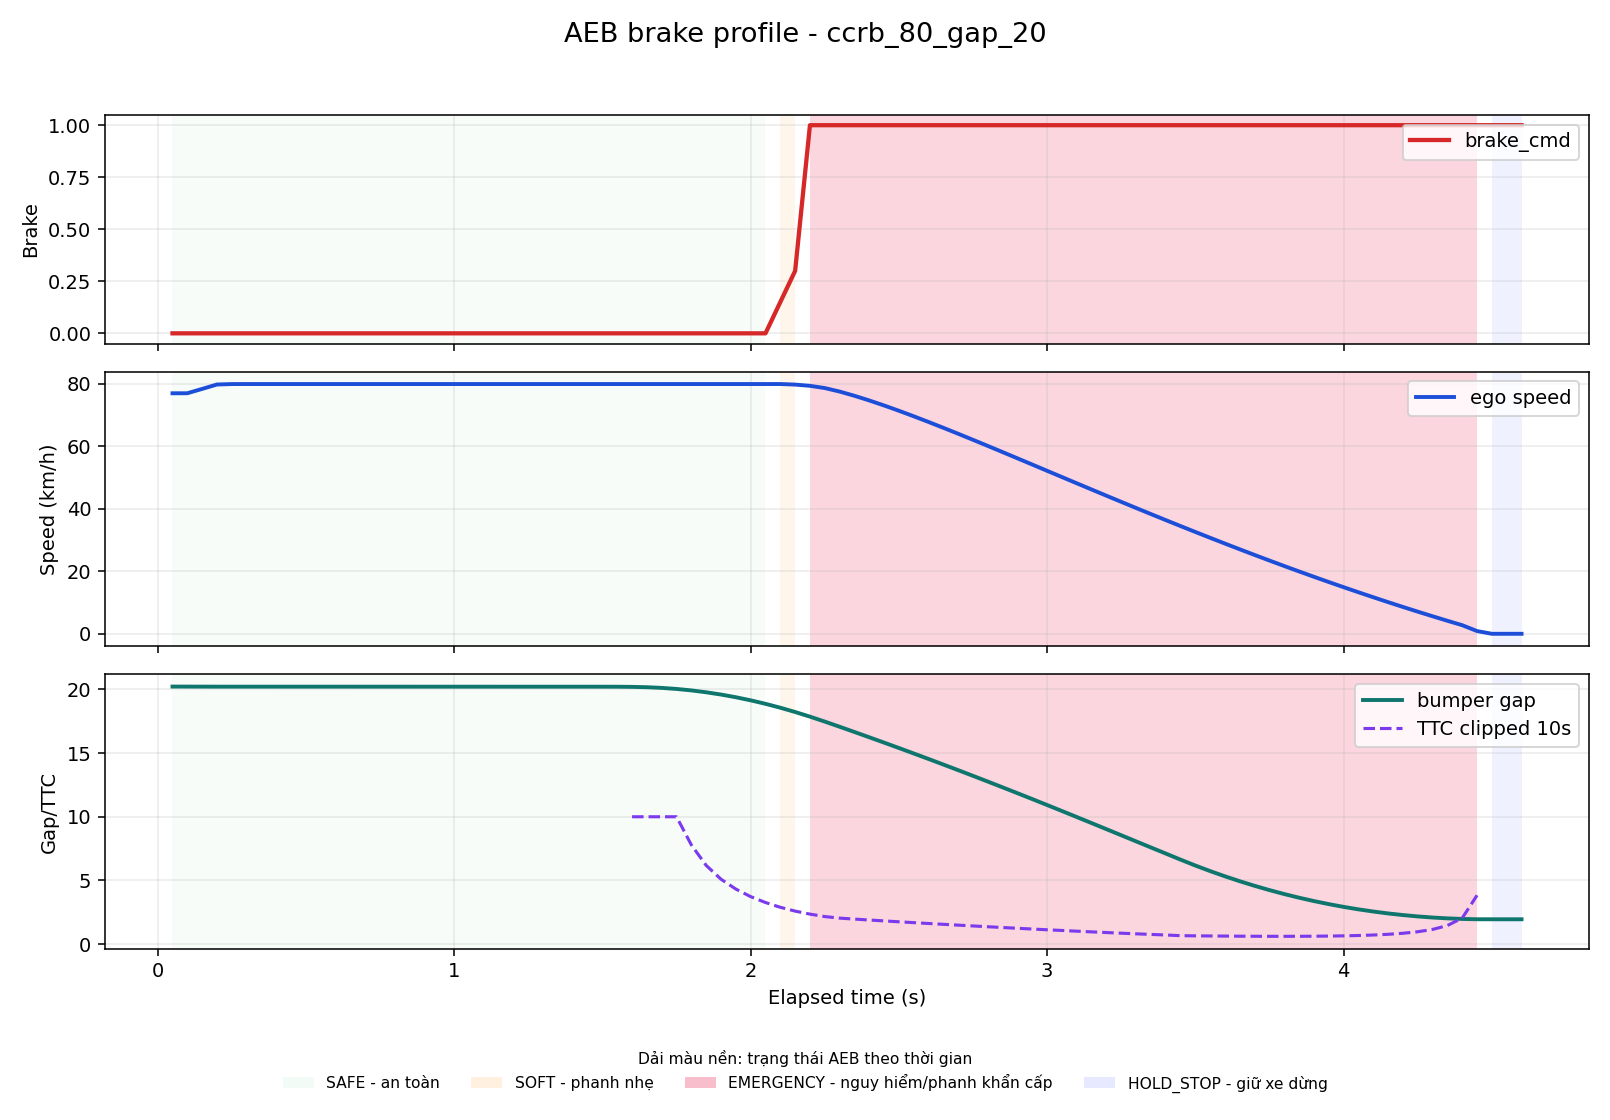
\includegraphics[width=0.49\columnwidth]{../../report/assets/evidence/brake_profile_ccrb_80_gap_20.png}
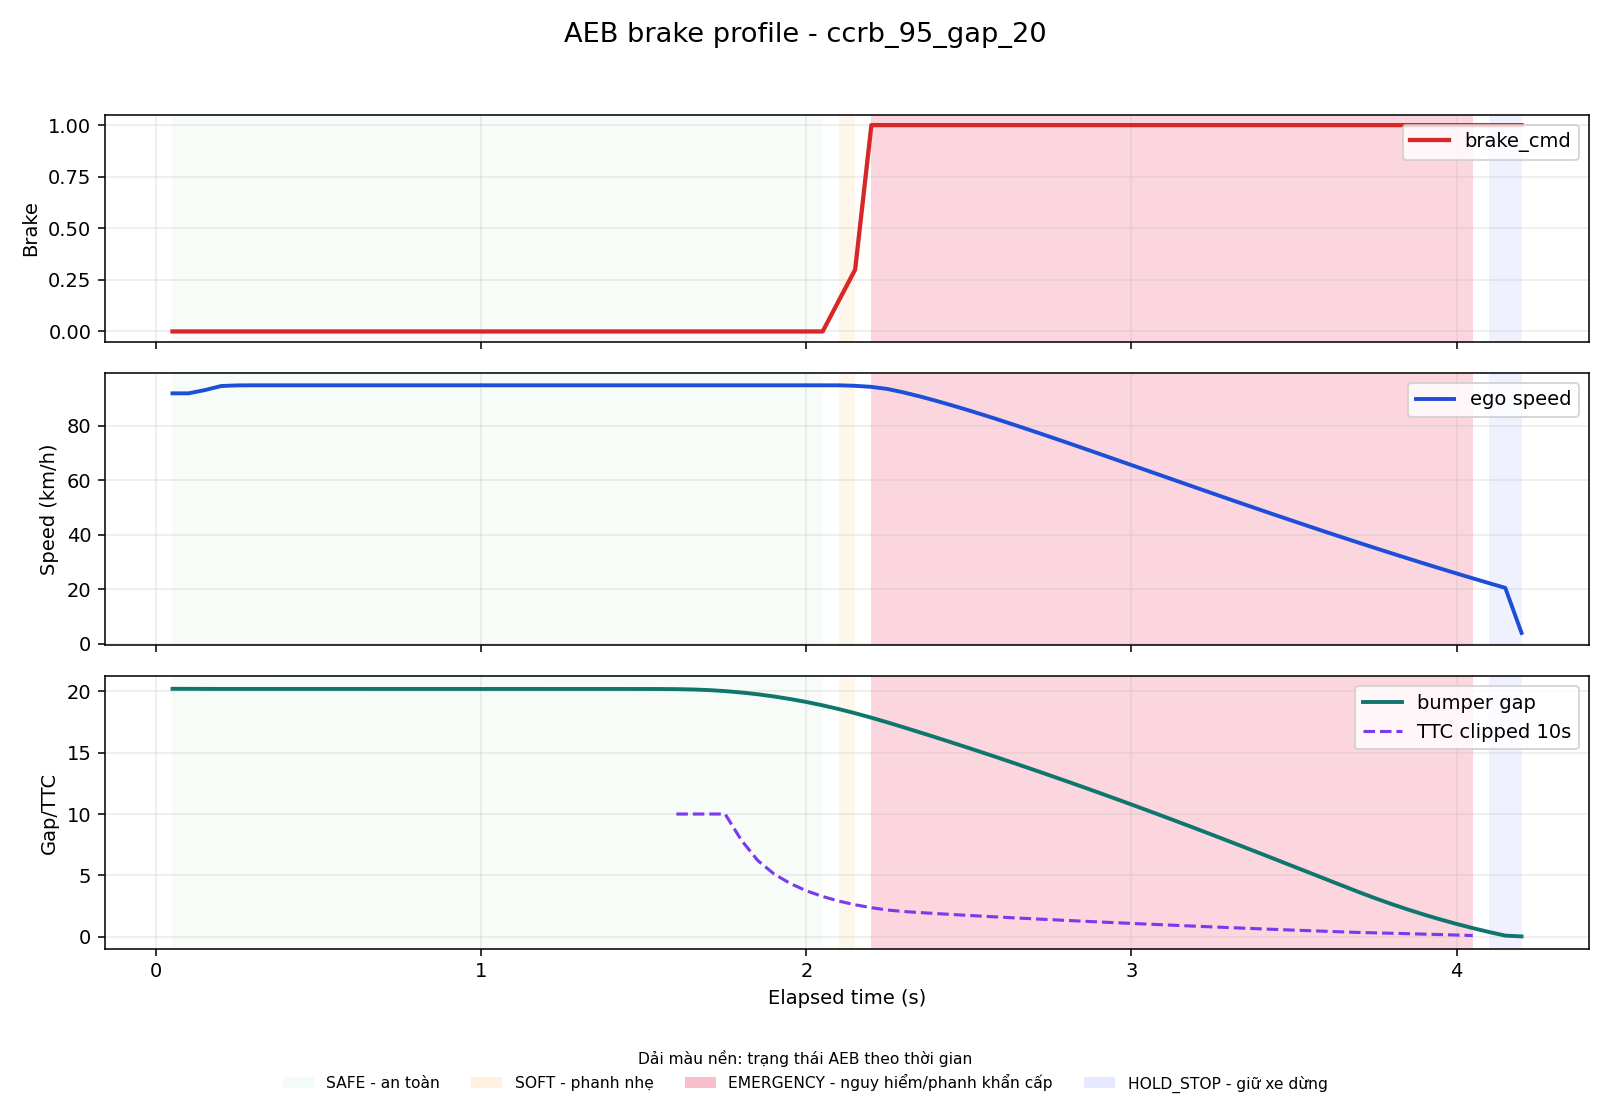
\includegraphics[width=0.49\columnwidth]{../../report/assets/evidence/brake_profile_ccrb_95_gap_20.png}
\caption{Biểu đồ phanh CCRb, gap đầu 20 m: đạt tại 80 km/h và va chạm tại 95 km/h.}
\label{fig:ccrb}
\end{figure}

Cut-in khó hơn vì target chỉ trở thành nguy hiểm khi đi vào hành lang ego. Ở case 80/50 km/h với gap đầu 25 m, phanh bắt đầu tại 10,46 m và khoảng cách nhỏ nhất còn 5,51 m. Ở case 100/60 km/h cùng gap, target được xác nhận muộn hơn; phanh bắt đầu tại 7,26 m và xảy ra va chạm, với min gap 0,476 m. Hai case minh họa giới hạn nhận thức--phản ứng của cấu hình một camera và một radar trong tình huống nhập làn nhanh.

\begin{figure}[t]
\centering
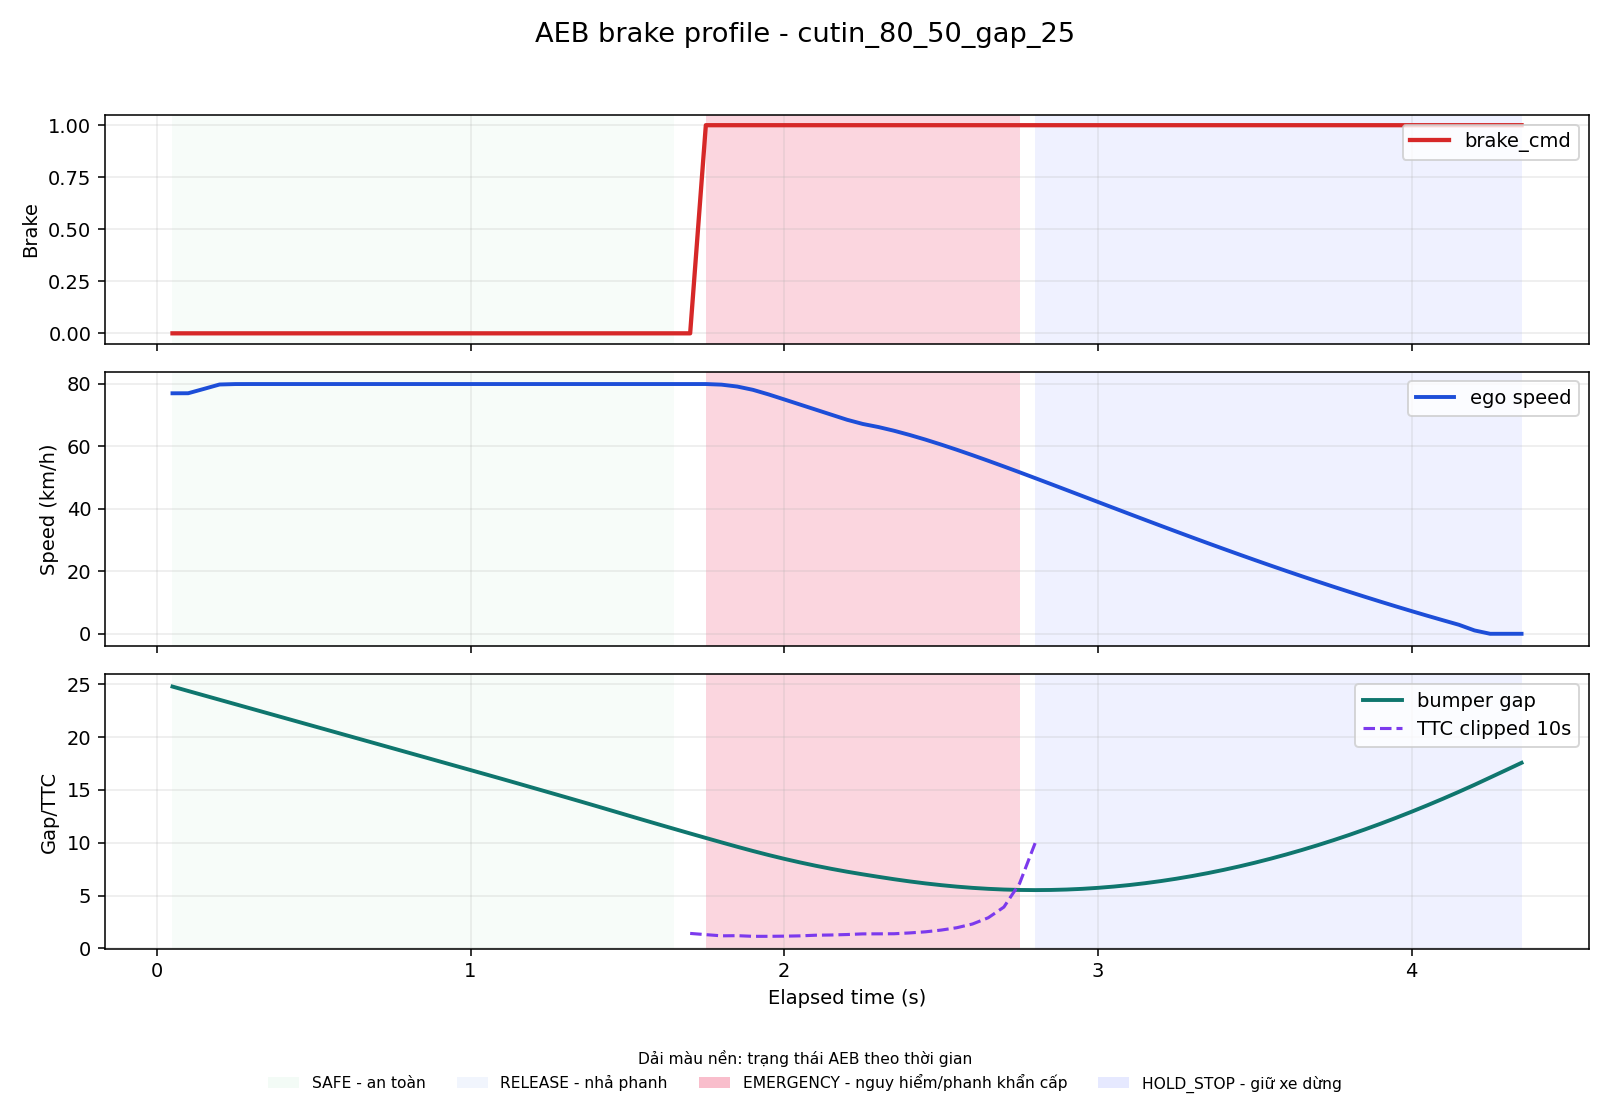
\includegraphics[width=0.49\columnwidth]{../../report/assets/evidence/brake_profile_cutin_80_50_gap_25.png}
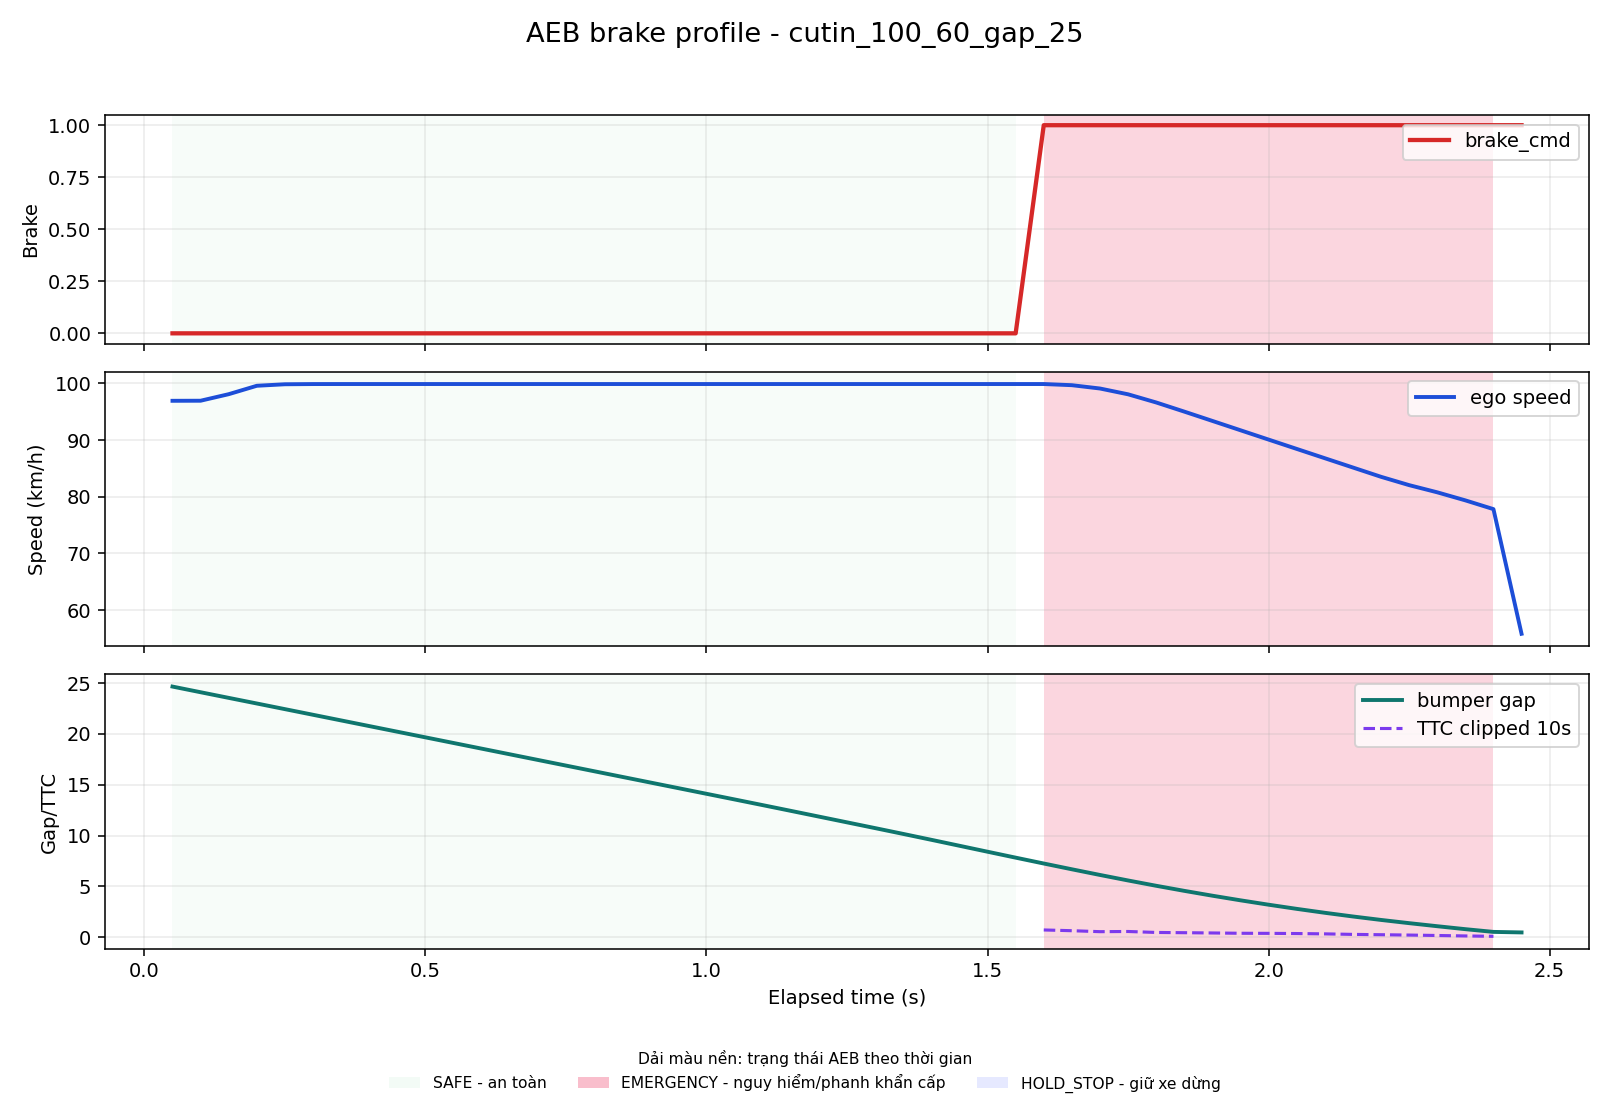
\includegraphics[width=0.49\columnwidth]{../../report/assets/evidence/brake_profile_cutin_100_60_gap_25.png}
\caption{Biểu đồ phanh cut-in: đạt tại 80/50 km/h và không đạt tại 100/60 km/h với gap đầu 25 m.}
\label{fig:cutin}
\end{figure}

Hình~\ref{fig:cutin} cho thấy đặc điểm riêng của cut-in: vùng nguy hiểm không tồn tại ngay từ đầu scenario như CCRs/CCRm/CCRb, mà hình thành khi xe làn bên cắt vào trước ego. Nếu gate hành lang quá rộng, AEB có thể phanh nhầm với xe làn bên; nếu gate quá hẹp hoặc xác nhận quá muộn, hệ thống thiếu thời gian phản ứng. Kết quả pass/fail của hai case cut-in cho thấy cấu hình hiện tại phù hợp ở 80/50 km/h nhưng chưa đủ ở 100/60 km/h khi target nhập làn gần.

Các case xe đứng yên làn bên, đường cong và nhiều xe bổ sung thông tin về false positive và chọn target. Một xe đứng yên ở làn bên trên đường cong không tạo lệnh phanh, trong khi xe đứng yên cùng làn vẫn được chọn và dừng với min gap 4,07 m. Với scenario nhiều xe có xe mồi làn bên, hệ thống bỏ qua xe mồi và phanh với xe chậm cùng làn. Như vậy, hành lang quỹ đạo, tracker và fusion gate có giá trị ngoài mục tiêu tránh va chạm đơn thuần.

Bộ final evidence hiện là đánh giá xác định theo simulator, chưa phải so sánh thống kê công bằng giữa các cấu hình. Trước khi nộp hội nghị, cần chạy lặp cùng seed cho radar-only, fusion-enabled và ít nhất một baseline điều khiển khác; báo cáo trung bình và độ lệch chuẩn của collision rate, false brake, min gap và first-brake distance. Jerk thô của CARLA chỉ dùng để so sánh tương đối trong cùng điều kiện vì đạo hàm gia tốc theo tick có thể có spike lớn.

\section{Kết luận}
Bài báo trình bày hệ thống AEB mô phỏng kết hợp radar mức đối tượng, YOLO camera, fusion gate hình học, hành lang quỹ đạo, TTC/khoảng cách dừng và staged PID. Hệ thống đạt 38/38 trong miền vận hành thiết kế và 63/66 trên tập kiểm thử gồm stress test. Ba case không đạt được giữ lại để xác định giới hạn tốc độ cao, gap ngắn và cut-in muộn. Hướng phát triển gồm lặp thí nghiệm có thống kê, mở rộng map/thời tiết/đối tượng, fusion xác suất có tracking đa mục tiêu, và mô hình hóa sâu hơn trễ actuator, bám đường và động lực học xe trước khi suy rộng sang xe thật.

\balance
\bibliographystyle{IEEEtran}
\bibliography{references}
\end{document}
